% Options for packages loaded elsewhere
\PassOptionsToPackage{unicode}{hyperref}
\PassOptionsToPackage{hyphens}{url}
%
\documentclass[
  12pt,
]{article}
\usepackage{lmodern}
\usepackage{amssymb,amsmath}
\usepackage{ifxetex,ifluatex}
\ifnum 0\ifxetex 1\fi\ifluatex 1\fi=0 % if pdftex
  \usepackage[T1]{fontenc}
  \usepackage[utf8]{inputenc}
  \usepackage{textcomp} % provide euro and other symbols
\else % if luatex or xetex
  \usepackage{unicode-math}
  \defaultfontfeatures{Scale=MatchLowercase}
  \defaultfontfeatures[\rmfamily]{Ligatures=TeX,Scale=1}
\fi
% Use upquote if available, for straight quotes in verbatim environments
\IfFileExists{upquote.sty}{\usepackage{upquote}}{}
\IfFileExists{microtype.sty}{% use microtype if available
  \usepackage[]{microtype}
  \UseMicrotypeSet[protrusion]{basicmath} % disable protrusion for tt fonts
}{}
\makeatletter
\@ifundefined{KOMAClassName}{% if non-KOMA class
  \IfFileExists{parskip.sty}{%
    \usepackage{parskip}
  }{% else
    \setlength{\parindent}{0pt}
    \setlength{\parskip}{6pt plus 2pt minus 1pt}}
}{% if KOMA class
  \KOMAoptions{parskip=half}}
\makeatother
\usepackage{xcolor}
\IfFileExists{xurl.sty}{\usepackage{xurl}}{} % add URL line breaks if available
\IfFileExists{bookmark.sty}{\usepackage{bookmark}}{\usepackage{hyperref}}
\hypersetup{
  hidelinks,
  pdfcreator={LaTeX via pandoc}}
\urlstyle{same} % disable monospaced font for URLs
\usepackage[margin = 1in]{geometry}
\usepackage{graphicx,grffile}
\makeatletter
\def\maxwidth{\ifdim\Gin@nat@width>\linewidth\linewidth\else\Gin@nat@width\fi}
\def\maxheight{\ifdim\Gin@nat@height>\textheight\textheight\else\Gin@nat@height\fi}
\makeatother
% Scale images if necessary, so that they will not overflow the page
% margins by default, and it is still possible to overwrite the defaults
% using explicit options in \includegraphics[width, height, ...]{}
\setkeys{Gin}{width=\maxwidth,height=\maxheight,keepaspectratio}
% Set default figure placement to htbp
\makeatletter
\def\fps@figure{htbp}
\makeatother
\setlength{\emergencystretch}{3em} % prevent overfull lines
\providecommand{\tightlist}{%
  \setlength{\itemsep}{0pt}\setlength{\parskip}{0pt}}
\setcounter{secnumdepth}{-\maxdimen} % remove section numbering
\usepackage{fancyhdr}
\pagestyle{fancy}
\lhead{\pagenumber}
\chead{}
\rhead{Applied Statistics}
\usepackage{setspace}
\doublespacing

\author{}
\date{\vspace{-2.5em}}

\begin{document}

\#School Performance

performance on math tests is determined by a wide range of factors.
These include a student's social class; educational stage, that is, the
grade a student is in; and gender. These factors have varying influences
on the students' performance in math. Being a crucial subject of study
at all levels of education, it is essential to leverage them into
improving the students' mathematical skills. In doing so, the school
board needs to determine the factors which impact the students'
performance on the math tests in the greatest way in order to prioritize
them. The scores in math tests can be modeled as a poisson model with
these factors as the parameters as follows:

\[ math ~ gender + socialclass + grade\]

Each of these factors takes a coefficient which corresponds to its
effect on the math score. In order to determine the most important
factor, this model was analyzed using Bayesian inference. The prior took
into consideration that the number of questions the student gets wrong
fits in a Poisson distribution. As such, a prior was taken for the
random effects incorporated in the model.

Although the results had a limited effectiveness due to the lack of a
relatively informed prior, the results held that the grade was the most
important factor affecting the performance of students in math tests. In
order to confirm this assessment, a histogram of the student's scores in
math tests were plotted in a histogram which highlighted differences
across grades. The results and the histogram suggested that students at
more advanced grades had a better grasp of the mathematical concepts
under study. As such, the school should develop a more effective method
of introducing the learners to mathematical concepts so that they can
grasp the ideas even at the lower grades.

The prior and posterior graphs are shown below.

\#Smoking

Smoking impairs the academic capability of students. In order to improve
the performance of students in a given area or institution, it is
essential to track and mitigate this behavior. To meet this goal, a
regression model was created using data from a large number of
demographically diverse students. After modelling it into a regression
model, Bayesian inference was used to determine whether the differences
in numbers of students who smoke were greater when comparing rural-urban
areas than across states. The regression model was:

\[y ~ β_1 sex+β_2  rural urban+ \varepsilon\]

In essence, the prevalence of smoking among students was determined by a
student's gender, since boys smoke more than girls; the influence of the
student's environment, which was under evaluation in this study; and
other random factors. The student's environment is an important
influence on a student's attitude towards smoking since it incorporates
the societal norms the student is subjected to. The Bayesian inference
assumed a neutral prior with a normal distribution. Based on input from
knowledgeable scientists in the field, the study also assumed that the
first hypothesis was true. In essence, the process of Bayesian inference
assumed that while the worst schools could only go as much as 50\% above
the best ones, the worst states could have rates as high as 5 to 10
times as much as the bet ones. As such, the inference compared the
prevalence of smoking in rural schools to urban ones. The R program for
the inference process produced a chart which highlighted a higher
prevalence in rural areas than in urban ones.

\begin{verbatim}
## 
## % Table created by stargazer v.5.2.2 by Marek Hlavac, Harvard University. E-mail: hlavac at fas.harvard.edu
## % Date and time: Tue, Nov 03, 2020 - 11:57:32 AM
## \begin{table}[!htbp] \centering 
##   \caption{} 
##   \label{} 
## \begin{tabular}{@{\extracolsep{5pt}}lccccccc} 
## \\[-1.8ex]\hline 
## \hline \\[-1.8ex] 
## Statistic & \multicolumn{1}{c}{N} & \multicolumn{1}{c}{Mean} & \multicolumn{1}{c}{St. Dev.} & \multicolumn{1}{c}{Min} & \multicolumn{1}{c}{Pctl(25)} & \multicolumn{1}{c}{Pctl(75)} & \multicolumn{1}{c}{Max} \\ 
## \hline \\[-1.8ex] 
## mean & 73 & 0.294 & 2.203 & $-$4.962 & $-$0.742 & 1.614 & 6.238 \\ 
## 0.025quant & 73 & $-$3.428 & 3.029 & $-$12.632 & $-$3.925 & $-$1.401 & $-$0.028 \\ 
## 0.975quant & 73 & 4.012 & 2.919 & $-$0.051 & 2.452 & 4.109 & 13.491 \\ 
## \hline \\[-1.8ex] 
## \end{tabular} 
## \end{table} 
## 
## % Table created by stargazer v.5.2.2 by Marek Hlavac, Harvard University. E-mail: hlavac at fas.harvard.edu
## % Date and time: Tue, Nov 03, 2020 - 11:57:32 AM
## \begin{table}[!htbp] \centering 
##   \caption{} 
##   \label{} 
## \begin{tabular}{@{\extracolsep{5pt}}lccccccc} 
## \\[-1.8ex]\hline 
## \hline \\[-1.8ex] 
## Statistic & \multicolumn{1}{c}{N} & \multicolumn{1}{c}{Mean} & \multicolumn{1}{c}{St. Dev.} & \multicolumn{1}{c}{Min} & \multicolumn{1}{c}{Pctl(25)} & \multicolumn{1}{c}{Pctl(75)} & \multicolumn{1}{c}{Max} \\ 
## \hline \\[-1.8ex] 
## mean & 1 & 0.406 &  & 0.406 & 0.406 & 0.406 & 0.406 \\ 
## 0.025quant & 1 & 0.301 &  & 0.301 & 0.301 & 0.301 & 0.301 \\ 
## 0.975quant & 1 & 0.546 &  & 0.546 & 0.546 & 0.546 & 0.546 \\ 
## \hline \\[-1.8ex] 
## \end{tabular} 
## \end{table}
\end{verbatim}

This backed the data obtained from the posterior quantiles. These
quantiles are shown in the table below:

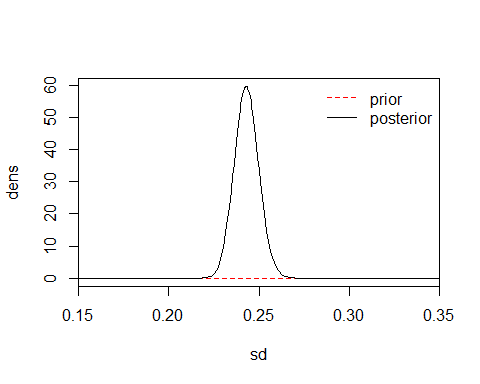
\includegraphics{homeworktwo_files/figure-latex/unnamed-chunk-2-1.pdf}

\hypertarget{appendices}{%
\section{Appendices}\label{appendices}}

\hypertarget{school-performance}{%
\subsection{School Performance}\label{school-performance}}

\begin{verbatim}

library(INLAutils)
library(INLA)
library(ggplot2)
library(tidyverse)
#load data

sUrl = "http://www.bristol.ac.uk/cmm/media/migrated/jsp.zip" 
dir.create(file.path("..", "data"), showWarnings = FALSE) 
(Pmisc::downloadIfOld(sUrl, file.path("..", "data")))

#create dataset from the info

school = read.fwf("../data/JSP.DAT", widths = c(2, 1, 1, 1, 2, 4, 2, 2, 1), 
                  col.names = c("school", "class", "gender", "socialClass", 
                                "ravensTest", "student", "english", "math", "year"))

#variables

school$socialClass = factor(school$socialClass, 
                            labels = c("I", "II", "IIIn", "IIIm", "IV", "V", 
                                       "longUnemp", "currUnemp", "absent"))
school$gender = factor(school$gender, labels = c("f", "m"))
school$classUnique = paste(school$school, school$class) 
school$studentUnique = paste(school$school, school$class,school$student)
school$grade = factor(school$year)

#generalized linear model

schoolLme = glmmTMB::glmmTMB(math ~ gender + socialClass + grade + (1 | school) + 
                               (1 | classUnique) + (1 | studentUnique), data = school)
summary(schoolLme)
knitr::kable(summary(schoolLme)$coef,digits = 3,caption = 'Regression Result')

#histogram

hist(1 - school$math,  breaks = 100)

#INLA

prec.prior <- list(prec = list(param = c(30, 0.05)))

mathscore = INLA::inla(math ~ gender + socialClass + grade+ f(
  data = school, model='iid', 
  hyper = prec.prior) +f(
    school, model='iid', 
    hyper = prec.prior), 
  data = school, control.predictor = list(compute = TRUE))

summary(mathscore)
knitr::kable(mathscore$summary.fixed, digits = 2, caption = "Posterior Quantiles")

#Plots of the original data
genderplot <- ggplot(school, aes(x= math, fill=gender, color=gender)) +
  geom_histogram(position="identity", binwidth=1, alpha=0.5) + labs(title = "Gender")

soclassplot <- ggplot(school, aes(x= math, fill=socialClass, color=socialClass)) +
  geom_histogram(position="identity", binwidth=1, alpha=0.5) + labs(title = "Socialclass")

gradeplot <- ggplot(school, aes(x= math, fill=grade, color=grade)) +
  geom_histogram(position="identity", binwidth=1, alpha=0.5) + labs(title = "Grade")

genderplot

soclassplot

gradeplot

#PLot of prior and posterior

sdRes = Pmisc::priorPostSd(mathscore)
do.call(matplot, sdRes$matplot)
do.call(legend, sdRes$legend)




\end{verbatim}

\hypertarget{smoking}{%
\subsection{Smoking}\label{smoking}}

\begin{verbatim}

#Load data
smokeFile=load("C:/Users/sa/Documents/MI205/smoke2014.RData")
smoke[1:3, c("Age", "ever_cigarettes", "Sex", "Race", "state", 
             "school", "RuralUrban")]

#Prepare data
forInla = smoke[smoke$Age > 10, c("Age", "ever_cigarettes", 
                                  "Sex", "Race", "state", "school", 
                                  "RuralUrban", "Harm_belief_of_chewing_to")]
forInla = na.omit(forInla)
forInla$y = as.numeric(forInla$ever_cigarettes)
forInla$ageFac = factor(as.numeric(as.character(forInla$Age))) 
forInla$chewingHarm = factor(forInla$Harm_belief_of_chewing_to,levels = 1:4, 
                             labels = c("less", "equal", "more", "dunno"))

#INLA
library("INLA")

toPredict = expand.grid(ageFac = levels(forInla$ageFac), 
                        RuralUrban = levels(forInla$RuralUrban), 
                        chewingHarm = levels(forInla$chewingHarm), 
                        Sex = levels(forInla$Sex))
forLincombs = do.call(inla.make.lincombs, 
                      as.data.frame(model.matrix(~Sex +ageFac * RuralUrban * chewingHarm, 
                                                 data = toPredict))) 
fitS2 = inla(y ~ Sex + ageFac * RuralUrban * chewingHarm + 
               f(state, model = "iid", hyper = list(prec = list(prior = "pc.prec", 
                                                                param = c(99, 0.05)))), 
             data = forInla, family = "binomial",control.inla = list(strategy = "gaussian"), 
             lincomb = forLincombs)

rbind(fitS2$summary.fixed[, c("mean", "0.025quant", "0.975quant")], 
      Pmisc::priorPostSd(fitS2)$summary[, c("mean", "0.025quant", "0.975quant")])
theCoef = exp(fitS2$summary.lincomb.derived[, c("0.5quant", "0.025quant", "0.975quant")])
theCoef = theCoef/(1 + theCoef)

toPredict$Age = as.numeric(as.character(toPredict$ageFac)) 
toPredict$shiftX = as.numeric(toPredict$chewingHarm)/10 
toPredict$x = toPredict$Age + toPredict$shiftX
toPlot = toPredict$Sex == "M" & toPredict$RuralUrban == "Rural"

plot(toPredict[toPlot, "x"], theCoef[toPlot, "0.5quant"], xlab = "age", 
     ylab = "probability", ylim = c(0,1), pch = 15, col = toPredict[toPlot, "chewingHarm"]) 

segments(toPredict[toPlot, "x"], theCoef[toPlot, "0.025quant"],
         y1 = theCoef[toPlot, "0.975quant"], col = toPredict[toPlot, "chewingHarm"])

legend("topleft", fill = 1:nlevels(toPredict$chewingHarm), 
       legend = levels(toPredict$chewingHarm), bty = "n", title = "chewing harmful")

\end{verbatim}

\end{document}
